\par A continuaci\'on se detallan todos los experimentos realizados en este
trabajo y sus resultados. Se detalla no s\'olo el experimento en si, sino que
tambi\'en se explican los resultados que se esperan comprobar y sus
motivaciones.

%---------------------------------------------------------------
\subsection{PageRank}
\subsection{Experimento 1}
\label{subsec:exp1}
\begin{LaTeXdescription}
    \item[Tesis]

    \item[Proposici\'on] 

    \item[M\'etodo de Experimentaci\'on]

    \item[Resultados, an\'alisis y discusi\'on]
\end{LaTeXdescription}


\newpage
\subsubsection{\'Ordenes: Google vs PageRank vs In-Deg}
\label{subsec:exp2}
\begin{LaTeXdescription}
    \item[Objetivo] Analizar el orden obtenido respecto de otros \'ordenes
        disponibles. ¿Es igual? ¿Hay coincidencias? ¿Cu\'antas? ¿Tienen
        sentido?\\

    \item[Proposici\'on] Cualitativamente hablando, ¿c\'omo es el orden obtenido
        por PageRank? ¿Bueno? ¿Malo?. Obviamente que estas categorizaciones son
        intr\'insecas a la realidad: s\'olo nosotros podemos decir que al
        realizar una b\'usqueda web, los resultados vinieron en un orden
        correcto o deseable (es decir, lo que se buscaba en las primeras
        posiciones).  Utilizar nuestro criterio personal para hablar de la
        calidad del orden obtenido no ser\'ia muy correcto, ya que cualquier
        otra persona con criterios distintos podr\'ia disentir y ninguno de los
        criterios ser\'ia \textit{a priori} m\'as correcto que el
        otro\footnote{Se podr\'ia ver muestralmente que opina la gente de
        distintos \'ambitos, pero esto escapa al objeto de estudio de este
        trabajo.}. Pero lo que si podemos hacer es comparar el resultado
        obtenido con otros resultados disponibles, de los cuales proponemos
        In-Deg (que se basa en el grafo de conectividad) y los resultados de un
        \textit{search engine}: Google.\\

    \item[M\'etodo de Experimentaci\'on] Utilizamos la misma instancia que en el
        experimento anterior. Sobre esta instancia s\'olo nos falta calcular el
        orden In-Deg (el cual no es otra cosa que ordenar a los nodos en orden
        descendiente seg\'un su grado de entrada, es decir seg\'un la cantidad
        de ejes que los apuntan). Luego utilizamos el orden provisto por Google
        en la b\'usqueda inicial m\'as los \'ordenes obtenidos en el experimento
        previo.\\

    \item[Resultados, an\'alisis y discusi\'on]
\end{LaTeXdescription}

\begin{table}[H]
    \centering
    \caption{\'Ordenes comparativos entre los resultados de Google, PageRank e
        In-Deg}
    \label{tbl:google_pagerank_vs_indeg_siteubaar} 
    \setlength{\tabcolsep}{3pt}
    \begin{tabular}{|l|l|l|}
        \hline
        Google & PageRank & In-Deg\\
        \hline\hline
        www.derecho.uba.ar & www.agro.uba.ar & www.agro.uba.ar\\
        orga2.exp.dc.uba.ar & www.uba.ar & www.uba.ar\\
        www.agro.uba.ar & videos.agro.uba.ar & videos.agro.uba.ar\\
        www.ffyb.uba.ar & www.agro.uba.ar/cursos & www.agro.uba.ar/cursos\\
        www.uba.ar & www.agro.uba.ar/ced & www.agro.uba.ar/ced\\
        www.fvet.uba.ar & www.derecho.uba.ar & www.derecho.com.ar\\
        videos.agro.uba.ar & www.ffyb.uba.ar & www.ffyb.uba.ar\\
        iigg.sociales.uba.ar & www.fvet.uba.ar & www.fvet.uba.ar\\
        www.agro.uba.ar/cursos & orga2.exp.dc.uba.ar & orga2.exp.dc.uba.ar\\
        www.agro.uba.ar/ced & iigg.sociales.uba.ar & iigg.sociales.uba.ar\\
        \hline
    \end{tabular}
\end{table}

\par Los resultados obtenidos en \ref{tbl:google_pagerank_vs_indeg_siteubaar}
dieron resultados idénticos en cuanto a In-Deg vs PageRank, no así la búsqueda
en google, que debe utilizar otras heurísticas que no consideramos en este
trabajo. Asimismo, el orden de las búsquedas en google para un mismo término van
cambiando a lo largo del tiempo\footnote{True Story.} .\\

\par Respecto a In-Deg y PageRank, sus \'ordenes resultaron idénticos. Los
motivos por lo cual esto ocurre fueron desarrollados en el experimento anterior,
pero intuyendo que esto no tiene que ser siempre
as\'i (sino claramente PageRank no tendr\'ia sentido), realizamos un nuevo
experimento. Creamos una nueva instancia de prueba basada en los resultados de
buscar en wikipedia\cite{wikipedia} distintos t\'erminos relacionados con los
temas vistos en la materia. El grafo de conectividad resultante se puede
observar en la figura \ref{fig:wiki_graph}.

\begin{figure}[H]
    \centering
    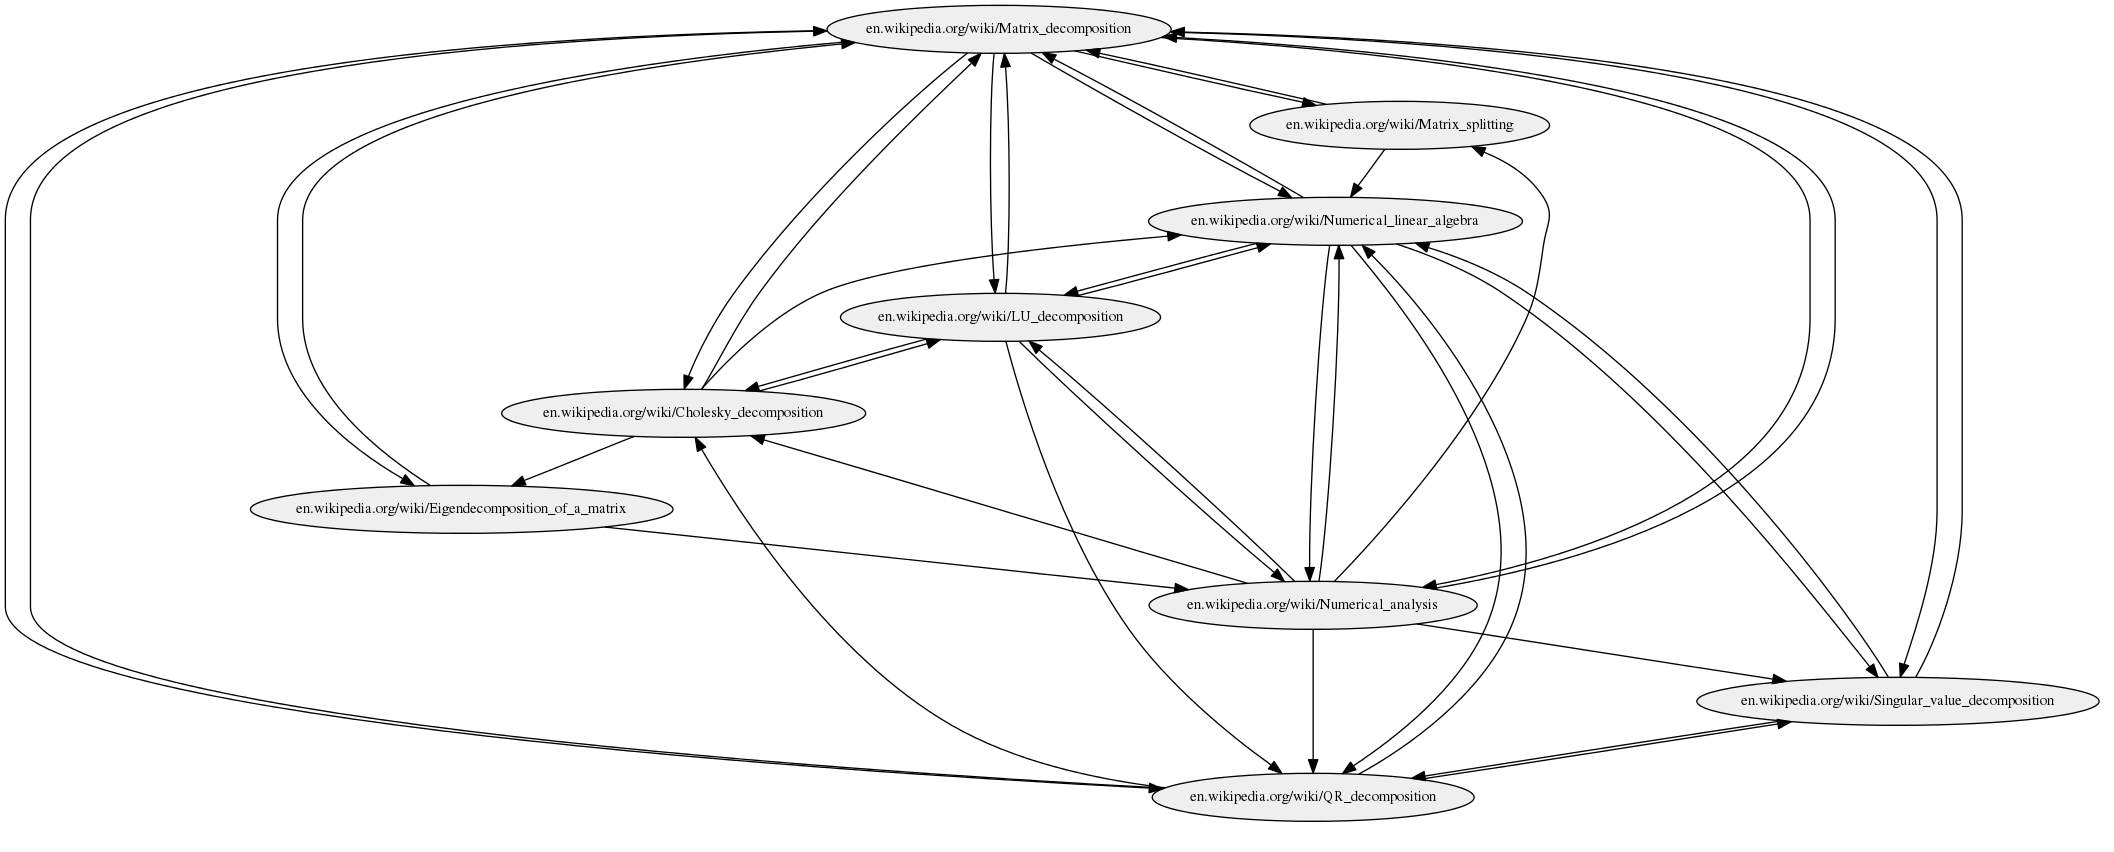
\includegraphics[width=0.75\textwidth]{exp2_conn_graph_metodos.png}
    \caption{Grafo de conectividad de p\'aginas de Wikipedia relacionadas con
        m\'etodos num\'ericos}
    \label{fig:wiki_graph}
\end{figure}

\par Sobre estas p\'aginas, calculamos los \'ordenes de PageRank e In-Deg, cuya
comparativa se encuentra detallada en el cuadro
\ref{tbl:pagerank_vs_indeg_wikipedia}. Nuevamente, In-Deg y PageRank dieron
resultados muy similares, pero no idénticos. M\'as aún, en In-Deg quedaron
varios nodos empatados, teniendo la misma cantidad de ejes entrantes. Pero esto
en PageRank no ocurri\'o, quedando definido un órden total.

\begin{table}[H]
    \centering
    \caption{\'Ordenes comparativos entre PageRank e In-Deg para Wikipedia}
    \label{tbl:pagerank_vs_indeg_wikipedia} 
    \setlength{\tabcolsep}{3pt}
    \begin{tabular}{|l|l||l|l|}
        \hline
        \multicolumn{2}{|c||}{PageRank} &\multicolumn{2}{c|}{In-Deg}\\
        \hline
        Puntaje & Nodo & Puntaje & Nodo\\
        \hline\hline
        0.196 & Matrix\_decomposition & 8 & Matrix\_decomposition\\
        0.165 & Numerical\_linear\_algebra & 7 & Numerical\_linear\_algebra\\
        0.125 & QR\_decomposition & 5 & QR\_decomposition\\
        0.106 & Numerical\_analysis & 4 & Numerical\_analysis\\
        0.105 & Singular\_value\_decomposition & 4 & LU\_decomposition\\
        0.098 & LU\_decomposition & 4 & Cholesky\_decomposition\\
        0.093 & Cholesky\_decomposition & 4 & Singular\_value\_decomposition\\
        0.057 & Eigendecomposition\_of\_a\_matrix & 2 & Eigendecomposition\_of\_a\_matrix\\
        0.050 & Matrix\_splitting & 2 & Matrix\_splitting\\
        \hline
    \end{tabular}
\end{table}

\par La diferencia entre \'ambos \'ordenes est\'a en la ubicaci\'on de
\emph{Singular value decomposition}. Mientras que en PageRank se encuentra en la
posici\'on 5, In-Deg lo lista en la 7ma ubicaci\'on. En el caso de In-Deg, la
determinaci\'on de la ubicaci\'on es determin\'istica, dependiendo del grado de
entrada del nodo que lo representa. Pero en nuestro ejemplo, vemos que existe un
empate con otros 3 nodos (como ya se ha explicado), con lo cual aqu\'i el orden
tambi\'en depende de la estabilidad y/o criterio de desempate que implemente
In-Deg. En nuestro caso, la implementaci\'on es estable, con lo cual se respeta
el orden inicial (o numeraci\'on) de los nodos. Por el otro lado, observando el
grafo podemos entender porque PageRank lo ubica en una posici\'on m\'as alta que
In-Deg: El nodo \emph{Numerical Linear Algebra}, uno de los de mayor puntaje (y
grado de entrada) tiene un link al nodo en cuesti\'on y a \emph{LU
decomposition}, pero no al resto de los valores que empatan en In-Deg. Por lo
visto en el experimento \ref{subsec:exp1}, sabemos que esto tiene un efecto de
subir el puntaje notoriamente en los nodos ''linkeados''. Luego, utilizando el
mismo razonamiento, observamos que \emph{Single value decomposition} queda por
encima de \emph{LU decomposition} por el voto/link de \emph{QR decomposition}.

\par Semánticamente, podemos observar que \textbf{en general}\footnote{\emph{QR}
queda por encima de \emph{Numerical Analysis}, creemos que esto se debe a la
morfología del grafo de referencias entre artículos en Wikipedia.} quedan
primeros en el ranking términos más \emph{generales} o \emph{abarcativos}; y a
medida que avanza el ranking se encuentran términos mas particulares.
Claramente, esta jerarqu\'ia de \emph{generalidad} es \'arbitraria para los
autores de este trabajo\footnote{¿Suma puntos hablar en tercera persona de
nosotros mismos? Very Scientific!}, aunque estimamos que habr\'a muy pocas
posibilidades de disenso al respecto para los temas representados por los nodos
del ejemplo.

\par Para evidenciar aún más la diferencia entre los algoritmos de In-Deg y
PageRank decidimos alterar expl\'icitamente el grafo de conectividad de este
\'ultimo ejemplo, agregando aristas desde los 5 nodos peor puntuados hacia uno
de los últimos en el ranking In-Deg (\emph{Eigendecomposition of a matrix}).
Esto deberia aumentar drásticamente el rankeo del ultimo elemento en In-Deg ya
que aumentamos su grado de entrada en 5, pero no tanto asi en Pagerank donde la
''calidad'' de los votantes tiene una mayor injerencia. Los resultados de este
último experimento pueden verse en el cuadro
\ref{tbl:pagerank_vs_indeg_wikipedia_modificado}. 

\begin{table}[H]
    \centering
    \caption{\'Ordenes comparativos entre PageRank e In-Deg para Wikipedia con grafo alterado explícitamente}
    \label{tbl:pagerank_vs_indeg_wikipedia_modificado}
    \setlength{\tabcolsep}{3pt}
    \begin{tabular}{|l|l||l|l|}
        \hline
        \multicolumn{2}{|c||}{PageRank} &\multicolumn{2}{c|}{In-Deg}\\
        \hline
        Puntaje & Nodo & Puntaje & Nodo\\
        \hline\hline
        0.189 & Matrix\_decomposition & 8 & Matrix\_decomposition\\
        0.137 & Numerical\_linear\_algebra & 7 & Numerical\_linear\_algebra\\
        0.123 & Numerical\_analysis & 7 & Eigendecomposition\_of\_a\_matrix\\
        0.114 & Eigendecomposition\_of\_a\_matrix & 5 & QR\_decomposition\\
        0.108 & QR\_decomposition & 4 & Numerical\_analysis\\
        0.097 & Singular\_value\_decomposition & 4 & LU\_decomposition\\
        0.089 & LU\_decomposition & 4 & Cholesky\_decomposition\\
        0.087 & Cholesky\_decomposition & 4 & Singular\_value\_decomposition\\
        0.051 & Matrix\_splitting & 2 & Matrix\_splitting\\
        \hline
    \end{tabular}
\end{table}

\par Puede observarse que respecto a In-Deg el elemento con ejes entrantes
artificiales paso a ser el
tercero por su nuevo grado de entrada aumentado. En Pagerank, el elemento subió
de ranking pero quedó por debajo de Numerical\_analysis, lo cual en principio es
raro, ya que este item quedó con puntaje 4 en In-Deg. Si miramos el grafo,
veremos que, efectivamente, el hecho de que \emph{Numerical analysis} sea apuntado por
\emph{Matrix decomposition} y \emph{Numerical linear algebra}, que son los términos mas
importantes, le da mas potencia al elemento en cuestión que al elemento
\emph{Eigendecomposition of a matrix}, apuntado por los últimos 5 de la lista.

%\par Por último, vemos que en el último experimento se acentúa el orden
%\texttt{abarcativo} de los resultados respecto al dominio de los elementos.

\medskip
\par A lo largo de este experimento pudimos evidenciar las diferencias que
existen entre dos algoritmos de elaboraci\'on de rankings distintos: In-Deg y
PageRank. Esto, que no lo hab\'iamos podido exponer en el experimento previo,
nos demostr\'o el peso que PageRank le otorga a los links provenientes de
p\'aginas web con mejores puntajes, diferenciaci\'on que In-Deg no realiza.
M\'as a\'un, nos encontramos conque In-Deg parece ser tener m\'as posibilidades
de empate en su forma de ''rankear'' que PageRank, volvi\'endose dependiente del
criterio de desempate que se utilice y convirti\'endose en otra
faceta/problema a resolver, situaci\'on que puede ser despreciada en el caso de
PageRank (las probabilidades de empate ya son chicas para pocos nodos, y las
mismas son cada vez menores a mayor cantidad). Como dato de color, observamos
que los resultados devueltos por \emph{Google} son bastante distintos de los
obtenidos con PageRank, con lo cual queda claro que a pesar de haber sido este
m\'etodo un hito en la historia del motor de b\'usqueda, el mismo ya a
evolucionado much\'isimo en pocos a\~nos, lo que demuestra la importancia del
problema estudiado. 


\newpage
\subsection{Convergencia de PageRank}
\label{subsec:exp3}
\begin{LaTeXdescription}
    \item[Objetivo] Estudiar como se comporta la convergencia en funci\'on de
        el factor de navegaci\'on $\alpha$.\\

    \item[Proposici\'on] PageRank propone una soluci\'on donde se observa a un
        conjunto de p\'aginas web como un grafo dirigido. Luego pasa este modelo
        a uno  matem\'atico, utilizando una matriz para computar una soluci\'on.
        Esta matriz, por construcci\'on, termina representando a un grafo
        completo (el grafo original no necesariamente lo era), y los valores del
        mismo dependen principalmente de 2 variables: $\epsilon$ y $\alpha$
        (algoritmo \ref{alg:power_method2}, p\'agina \pageref{alg:power_method2}
        y ecuaci\'on \ref{eq:M_def}, p\'agina \pageref{eq:M_def}). Si se observa
        el algoritmo, se ver\'a que claramente modificar el $\epsilon$ tendr\'a
        como resultado hacer que cada corrida converja en m\'as o menos
        iteraciones, ya que el criterio de parada depende de \'el. As\'i pues,
        no vemos como algo rico experimentar con este valor. En cambio, $\alpha$
        es una variable que modifica en gran medida a nuestra matriz $M$, con lo
        cual es dificil saber cual ser\'a su injerencia en la convergencia (en
        principio). El objetivo, entonces, es ver como $\alpha$ afecta al
        m\'etodo matem\'atico iterativo de la potencia en cuanto a su
        convergencia.\\

    \item[M\'etodo de Experimentaci\'on] Tomaremos 3 instancias de grafos de
        conectividad de p\'aginas web de tama\~no mediano-grande, obtenidas en
        \url{http://snap.stanford.edu/data/\#web}. Luego, correremos el
        algoritmo de PageRank para $\alpha=0.0$; $0.1$; $0.2$; $\dots$; $0.9$ y
        $\epsilon$ fijo en $0.00001$.\\

    \item[Resultados, an\'alisis y discusi\'on]
\end{LaTeXdescription}

\par En el gráfico \ref{subfig:exp3_comp} se exponen la cantidad de iteraciones
necesarias hasta converger a medida que el parámetro $\alpha$ crece. Para las 3
instancias el comportamiento observado es el mismo: a medida que el par\'ametro
$\alpha$ aumenta, la cantidad de iteraciones necesarias para converger crece
exponencialmente. Puede observarse que aunque con valores numéricos diferentes,
las curvas pertenecen a la misma familia de funciones, y por lo tanto tienen un
comportamiento id\'entico (emp\'iricamente hablando) en cuanto a la cantidad de
iteraciones en funci\'on de $\alpha$.

\begin{figure}[H]
    \centering
    \caption{An\'alisis de Convergencia en funci\'on de $\alpha$}
    \subfloat[][Iteraciones hasta Converger en funci\'on de $\alpha$]{
        \label{subfig:exp3_comp}
        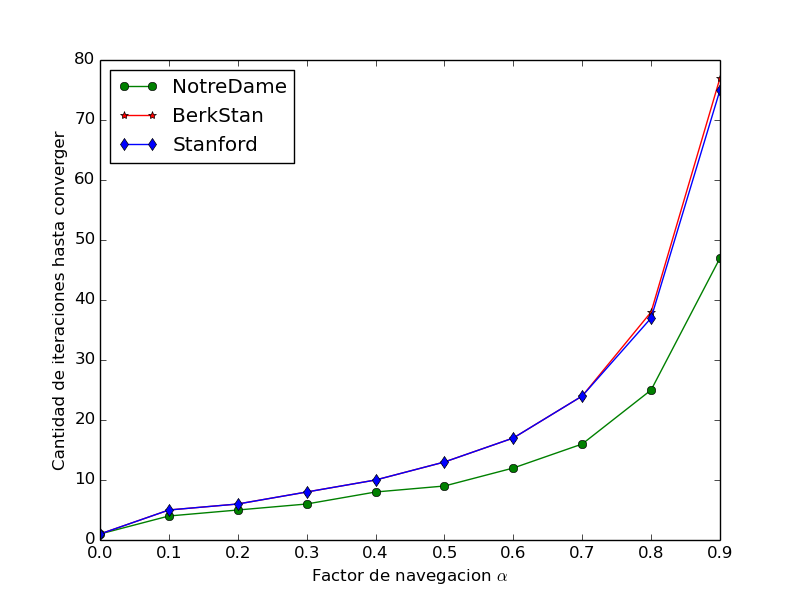
\includegraphics[width=.5\textwidth]{exp3_iteraciones_funcion_alpha.png}
    }
    \subfloat[][Velocidad de convergencia en funci\'on de $\alpha$\\Escala
    logar\'itmica]{
        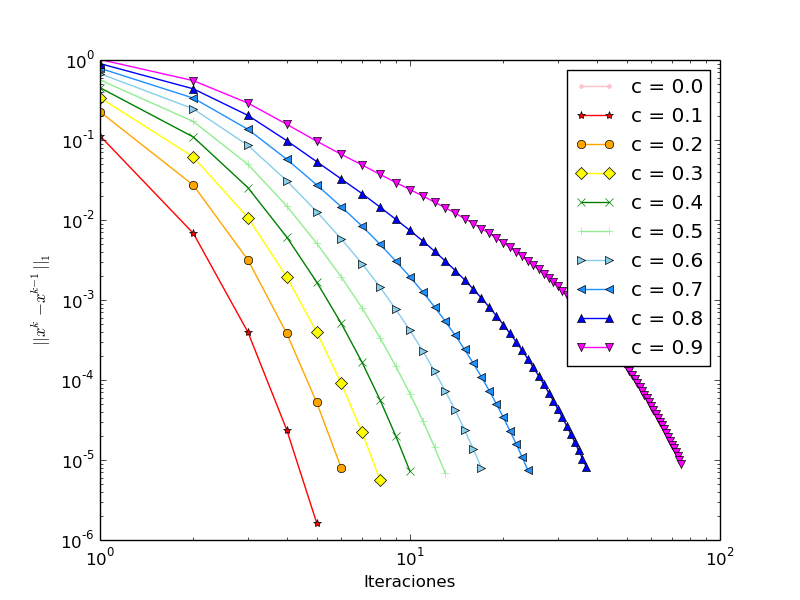
\includegraphics[width=.5\textwidth]{exp3_diff_funcion_iteraciones_standford.png}
        \label{subfig:exp3_diff}
    }
\end{figure}

\par Como se explic\'o en la secci\'on \ref{sec:introduccion}, el factor
$\alpha$ hace variar la proporci\'on entre $S$ y la matriz equiprobable a la
hora de definir a $M$. Es decir, en el rango de posibles valores de $\alpha$, la
\'unica manera en la que se afecta a $M$ es en los valores de cada uno de sus
elementos. Pero para ning\'un $\alpha$ se puede pasar a tener un elemento nulo
en $M$ (justamente se quer\'ia tener la representaci\'on de un digrafo
completo). As\'i pues, la pregunta pasa a ser: ¿Por qu\'e a mayor $\alpha$ se
necesitan m\'as iteraciones para converger?

\par Se nos ocurre que, volviendo al contexto de una cadena de Markov y el
navegante aleatorio, un $\alpha$ peque\~no nos genera una matriz de transici\'on
''m\'as'' equiprobable (recordar la definici\'on de $M$ en la ecuaci\'on
\ref{eq:M_def}, p\'agina \pageref{eq:M_def}) y dado que el método de la potencia
comienza inicialmente con el vector equiprobable, le toma pocas iteraciones
converger. A medida que $\alpha$ aumenta, el grafo generado denota más la
navegación estricta por los links entre los sitios, reduciendo la probabilidad
de teletransportación. Es decir, a mayor $\alpha$, el grafo se ''parece m\'as''
al grafo de conectividad original no adulterado (con los dangling nodes ya
resueltos), en el sentido de que $S$ predomina mucho m\'as en $M$ que
$(\rfrac{1}{n})ee^T$. Esta matriz $S$ no necesariamente representa un grafo
fuertemente conexo, una de las condiciones necesarias para asegurar convergencia
del método de la potencia en el contexto de este problema, con lo cual el método
de la potencia inicia sus iteraciones con una, si se quiere, \textbf{seguridad
de convergencia más débil}.

\par Respecto a la velocidad de convergencia, exponemos los resultados de una
sola instancia ya que para las 3 instancias los resultados son similares. Como
puede observarse en el gráfico \ref{subfig:exp3_diff}, a medida que el factor de
navegacion $\alpha$ crece, la velocidad de convergencia disminuye,
obteni\'endose curvas cada vez m\'as pronunciadas.

\par La ''velocidad de convergencia'' la definimos como la distancia
\emph{Manhattan} entre los autovectores $\vec{x^{(k)}}$ y $\vec{x^{(k-1)}}$
calculados en dos iteraciones consecutivas. Mientras mayor sea la distancia,
m\'as r\'apido decimos que se converge\footnote{Asumiendo que $\vec{x^{(k)}} <
\vec{x^{(k-1)}}$, caso contrario nos estar\'iamos alejando del criterio de corte
del m\'etodo, es decir, de converger.}, pues se est\'a acerc\'andose cada vez
\textbf{m\'as rápido} al umbral de corte del algoritmo (basado en $\epsilon$ o
una cantidad fija m\'axima de iteraciones\footnote{Esto se implementa, ya que si
bien la teor\'ia nos indica que el m\'etodo convergir\'a, los errores
n\'umericos de la aritm\'etica finita puede hacer que esto no ocurra.}).

\par Nuestra explicaci\'on para este comportamiento es exactamente la misma que
se expuso para el caso de las iteraciones hasta converger en funci\'on de
$\alpha$. Sin ir m\'as lejos, estamos hablando del mismo fen\'omeno, salvo que
en el caso de la figura \ref{subfig:exp3_diff} hacemos hincapi\'e en
\textbf{como} se acerca el m\'etodo al vector soluci\'on, mientras que en la figura
\ref{subfig:exp3_comp} observamos m\'as en detalle la \textbf{cantidad de
iteraciones} que se necesitan. Sin embargo, ambos gr\'aficos nos muestran lo
mismo: \textit{a que velocidad}, o \textit{cuanto tiempo/iteraciones} se
requieren para converger en funci\'on de $\alpha$.

\par Ahora bien, hemos visto como $\alpha$ afecta a la convergencia. S\'i esto
fuera lo \'unico, claramente siempre elegir\'iamos el valor que nos permita
converger m\'as r\'apido. Ocurre que, como vimos en el experimento
\ref{subsec:exp1}, el $\alpha$ afecta al orden obtenido tambi\'en, es decir, a
la calidad del resultado. As\'i pues, la elecci\'on de este par\'ametro ser\'a
la b\'usqueda del equilibrio \emph{efectividad} y \emph{eficiencia}, u entre
calidad del resultado y ti\'empo de c\'omputo (intuitivamente, m\'as iteraciones
implican mayor tiempo de c\'omputo). La bibliograf\'ia consultada nos indica que
en su momento, Google fij\'o inicialmente este par\'ametro en $0.85$,
considerando a este un \emph{trade-off} lo suficientemente
bueno\cite{Bryan2006}\cite{Langville2006}.

\par As\'i pues conclu\'imos nuestra experimentaci\'on sobre la convergencia del
m\'etodo de la potencia para PageRank. Llegamos a un resultado inmediato que nos
dice que a mayor $\alpha$ tendremos una velocidad de convergencia menor y, ergo,
una cantidad de iteraciones necesaria mayor para obtener un resultado lo
suficientemente apr\'oximado. Tambi\'en evaluamos brevemente la contracara de
tener un tiempo de convergencia chico: el resultado obtenido no necesariamente
es el mismo ya que predomina m\'as la equiprobabilidad de los ejes de
teletransportaci\'on artificalmente a\~nadidos a la matr\'iz $M$. Tambi\'en
obtuvimos como resultado que este comportamiento es, presumiblemente (har\'ia un
falta un an\'alisis m\'as minucioso para poder afirmarlo), el mismo para
cualquier instancia de entrada, m\'as all\'a de que la cantidad de iteraciones
absoluta entre dos instancias pueda variar para el mismo $\alpha$, el
comportamiento en funci\'on de $\alpha$ parecer\'ia ser el mismo.


\newpage
\subsection{An\'alisis de Tiempo de C\'omputo}
\label{subsec:exp4}
\begin{LaTeXdescription}
    \item[Objetivo] Analizar la complejidad temporal del m\'etodo.\\

    \item[Hip\'otesis] Proponemos que el tiempo de c\'omputo por iteraci\'on
        para una instancia y $\epsilon$ fijos ser\'a siempre el mismo para todo
        $\alpha$. Tambi\'en proponemos que el tiempo de c\'omputo por interación
        para $\epsilon$ fijo ser\'a el mismo para \textbf{toda instancia} (sin
        importar tama\~no, cantidad de ejes, etc).\\

    \item[Proposici\'on] De los experimentos previo hemos llegado a la
        conclusi\'on de que a mayor $\alpha$, mayor cantidad de iteraciones
        ser\'an necesarias para converger, lo cual implica inmediatamente un
        mayor tiempo de c\'omputo requerido. La pregunta ideal a responder
        ser\'ia ''cu\'anto tiempo'', pero tambi\'en concluimos previamente que
        la cantidad de iteraciones es dependiente (entre otros factores) de la
        instancia de entrada. Con lo cual, responder a esta pregunta en el
        contexto de este trabajo es imposible sin una cota te\'orica para la
        cantidad de iteraciones (que ni siquiera sabemos si existe). En cambio,
        lo que s\'i podemos analizar es si el tiempo de c\'omputo \textbf{por
        iteraci\'on} es el mismo para toda instancia, sin importar el
        $\epsilon$\footnote{M\'as all\'a de para nuestros experimentos lo
        estemos dejando fijo.} o $\alpha$. Analizamos entonces si el tiempo por
        iteraci\'on var\'ia seg\'un la densidad de la instancia inicial, y a su
        vez si varía para distintos valores de $\alpha$.\\

    \item[M\'etodo de Experimentaci\'on] Tomamos 3 instancias de tama\~no
        mediano-grande, con una diferencia relativa de densidad entre ellas
        significativa. Particularmente, tomamos las mismas del experimento
        anterior. Luego resolvemos cada instancia con PageRank 10 veces para
        $\alpha=0.0$; $0.1$; $0.2$; $\dots$; $0.9$\footnote{Totalizando un total
        de 300 corridas del m\'etodo (10 corridas para 10 valores de $\alpha$
        para 3 instancias distintas).}. Tomamos entonces para cada instancia y
        $\alpha$ fijos, el promedio de los tiempos de c\'omputo. Por \'ultimo,
        calculamos el tiempo de c\'omputo por iteraci\'on dividiendo este
        promedio por la cantidad de iteraciones totales que necesit\'o el
        m\'etodo para converger.\\

    \item[Resultados, an\'alisis y discusi\'on]
\end{LaTeXdescription}

\par Consideramos 2 enfoques para extraer conclusiones, el primero analiza el
tiempo consumido por iteración por el método de la potencia para diferentes
valores de $\alpha$ y el segundo se centra en el tiempo por iteraci\'on respecto
de la densidad de la instancia/grafo de entrada\footnote{Al referirnos a
\emph{densidad} de un grafo, nos referimos a la cantidad de ejes que tiene. A
mayor cantidad de ejes, m\'as denso es.}.

\begin{figure}[H]
    \centering
    \caption{An\'alisis de Tiempo de C\'omputo} %en funci\'on de $\alpha$}
    \subfloat[][Tiempo por Iteraci\'on en funci\'on de $\alpha$.]{
        \label{subfig:exp4_tiempo_iteracion}
        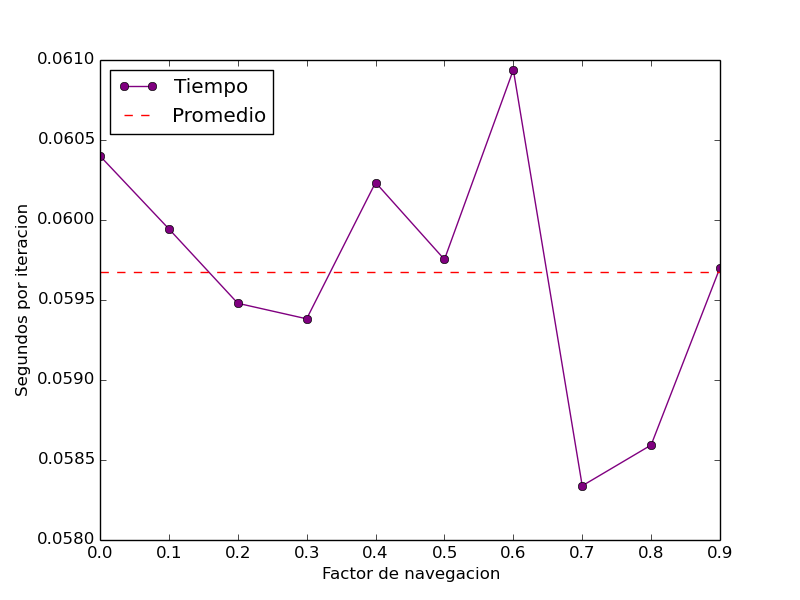
\includegraphics[width=.55\textwidth]{exp4_tiempo_por_iteracion_notredame.png}
    }
    %\begin{figure}[H]
    %    \centering
        \subfloat[][Tiempo por Iteraci\'on promedio vs Densidad del Grafo]{
            \label{subfig:exp4_den}
            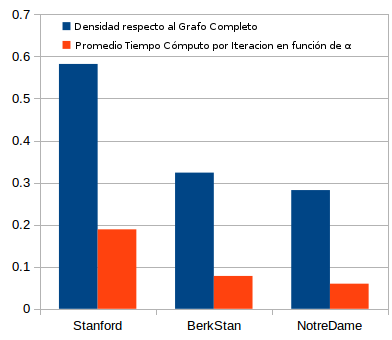
\includegraphics[width=.45\textwidth]{exp4_tiempo_vs_densidad.png}
        }
        %\caption{An\'alisis de Tiempo de C\'omputo en funci\'on de la densidad del Grafo}
    %\end{figure}
    %\subfloat[][Tiempo por Iteraci\'on en funci\'on de $\alpha$. Escala logarítmica]{
    %    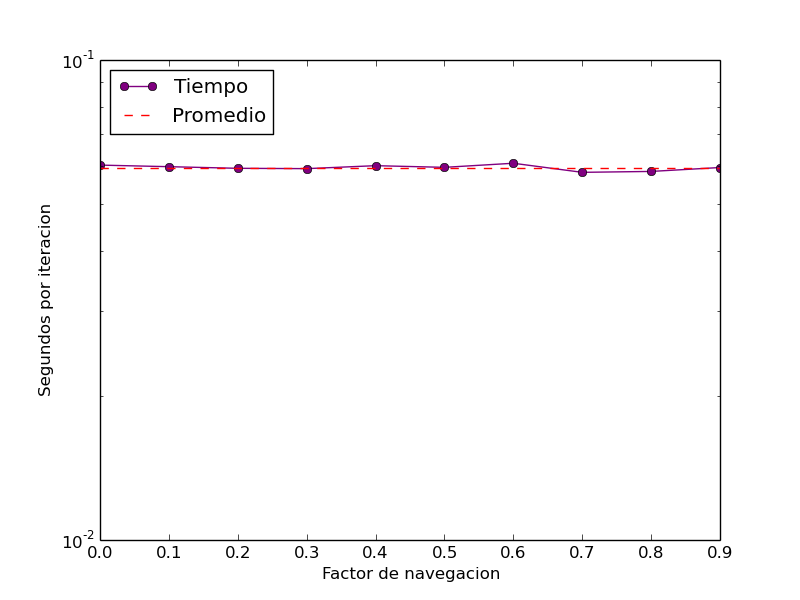
\includegraphics[width=.45\textwidth]{exp4_tiempo_por_iteracion_notredame_log.png}
    %    \label{subfig:exp4_tiempo_iteracion_log}
    %}
\end{figure}

\par Para el primer enfoque, observemos los resultados obtenidos en la figura
\ref{subfig:exp4_tiempo_iteracion}. En el mismo observamos dos curvas. La
primera, \emph{Tiempo}, que representa el tiempo por iteraci\'on promedio para
cada $\alpha$ (calculado como el tiempo promedio hasta converger de las 10
ejecuciones para un $\alpha$ fijo, dividido por la cantidad de iteraciones que
necesit\'o); y la segunda \emph{Promedio} que no es otra cosa que el promedio de
los tiempos por iteraci\'on calculados para la curva \emph{Tiempo}. Los
resultados expuestos en esta figura son similares para las 3 instancias de
prueba que se tomaron, con lo cual se decidi\'o exponer una sola.

\par Puede observarse en esta misma figura que el tiempo por iteraci\'on
calculado en funci\'on de $\alpha$ oscila en valores muy pequeños alrededor del
promedio. Para ilustrar esto, presentamos en el cuadro
\ref{tbl:exp4_data_notredame} las m\'etricas empíricas del experimento.

\begin{table}[H]
    \centering
    \caption{Métricas del tiempo por iteracion respecto de $\alpha$}
    \label{tbl:exp4_data_notredame} 
    \setlength{\tabcolsep}{3pt}
    \begin{tabular}{|l|l|}
        \hline
        Métrica & Segs\\
        \hline\hline
        Promedio & 0.059676\\
        Desv\'io Est\'andar & 0.000788\\
        M\'inimo & 0.058338\\
        M\'aximo & 0.060938\\
        Diferencia \%\footnotemark& 4.266231\\
        \hline
    \end{tabular}
\end{table}
\footnotetext{Diferencia \%: 100*(max-min)/max.}


\par Estas variaciones seguramente se deben al \emph{scheduler} del sistema
operativo y a fenómenos de bajo nivel de las corridas de los
experimentos. De hecho, ya vimos en el experimento \ref{subsec:exp3} que a
medida que aumentamos el $\alpha$, m\'as iteraciones ser\'an necesarias para
converger. Obviamente esto implica un mayor tiempo de c\'omputo, ergo, la
ejecuci\'on del experimento se vuelve a\'un m\'as sensible pues al estar m\'as
tiempo ejecut\'andose m\'as probabilidades hay de que el Sistema Operativo
decida darle el CPU a otro proceso de mayor prioridad que surja (o que al estar
tanto tiempo ejecut\'andose, su prioridad vaya bajando).

\par Finalmente conclu\'imos que que el tiempo por iteraci\'on es constante, ya
que en las m\'etricas nos confirman, al observar los valores muy peque\~nos del
desv\'io est\'andard y diferencia porcentual, que estas diferencias para
distintos $\alpha$ sean muy probablemente errores de medici\'on (recordemos que
adem\'as estamos trabajando con instancias de entrada de tama\~no
mediano-grande).

\par Habiendo llegado a la conclusi\'on que la hip\'otesis sobre el tiempo de
c\'omputo por iteraci\'on es constante, debemos analizar por qu\'e. Repasando la
secci\'on \ref{sec:implementacion}, podemos decir que es razonable el
comportamiento presupuesto y observado, ya que el valor de $\alpha$ no modifica
la \emph{densidad} de la matriz original de conectividad $A$. Recordemos
entonces que nuestra implementaci\'on se basa en el algoritmo
\ref{alg:power_method3}, p\'agina \pageref{alg:power_method3}, que multiplica
usando justamente esta matriz $A$ y aprovechando que la misma es esparsa. Al no
modificar esta caracter\'istica la selecci\'on del par\'ametro $\alpha$, podemos
afirmar que la cantidad de $flops$ necesarios para el producto matriz-vector se
mantendr\'a constante en funci\'on de $\alpha$ (de hecho, $\alpha$ es un
par\'ametro que luego multiplica al vector resultante $A\vec{x}^{(k-1)}$ en
nuestro algoritmo, con lo cual no afecta en lo absoluto al producto
matriz-vector que involucra a $A$).

\par El segundo enfoque centra su atención en el tiempo por
iteracion respecto a la densidad del grafo asociado a la instancia de entrada.
Al contrario que lo esperado, la densidad (cantidad de ejes) del
grafo \textbf{s\'i} altera el tiempo de cómputo por iteración. Si observamos la
figura \ref{subfig:exp4_den}, observaremos que a mayor densidad, mayor tiempo
por iteraci\'on se necesita.

\par En esta figura se compara el tiempo promedio consumido\footnote{Se utiliza
el valor promedio del tiempo para todos los factores de navegación.} contra una
medida de densidad del grafo\footnote{Se toma como métrica un cociente entre la
cantidad de aristas del gráfo y la cantidad de aristas de una \emph{clique} de
su misma cantidad de nodos; multiplicado por una constante para igualar las
magnitudes con los valores de los tiempos de c\'omputo.}, y se v\'e, para las 3
instancias evaluadas, que el crecimiento del tiempo de c\'omputo parecer\'ia ser
l\'ineal en funci\'onde la densidad del grafo. Dado que s\'olo experimentamos
con estas 3 instancias, ser\'ia muy abrupto hacer dicha afirmaci\'on, pero si
podemos decir que tenemos sospechas de que eso ocurra, dejando este aspecto para
un futuro posible experimento\footnote{Vale la pena aclarar, en este caso, que
podr\'iamos considerar a nuestras 3 instancias como poco densas, m\'as alla de
la diferencia notoria de densidad entre ellas.}.

\par Volviendo al hecho de que a mayor densidad, mayor ti\'empo de c\'omputo,
llegamos a la conclusi\'on de que esto se debe al mismo motivo que en el primer
enfoque, salvo que esta vez justifica el hecho de que \textbf{s\'i} se requiera
m\'as tiempo de c\'omputo. Ocurre que al ser la instancia de entrada m\'as
densa, menos esparsa ser\'a $A$ (m\'as ejes implica mayor cantidad de valores no
nulos en la matriz), y por lo tanto el producto $A\vec{x}$ de la
implementaci\'on del m\'etodo efectuar\'a m\'as $flops$.

\medskip
\par Finalizando, concluimos que 1 de nuestras hip\'otesis era correcta, y la
otra no. Peculiar es, que las justificaciones que le encontramos a ambos
comportamientos (la relaci\'on tiempo de c\'omputo por iteraci\'on en funci\'on
de $\alpha$ y de la densidad de la instancia) es la misma: mientras que $\alpha$
no afecta a la densidad de la matriz de conectividad pesada $A$, cosa que si lo
hace la cantidad de ejes del grafo. Es decir, terminamos entendiendo que el
principal aspecto a tener en cuenta a la hora de ver como se ver\'a afectado el
tiempo de computo (para nuestra implementaci\'on basada en el algoritmo
propuesto por Kamvar et al.\cite{Kamvar2003}) ser\'a la
densidad/esparcidad\footnote{Coloquialismo.} de la matriz inicial del modelo.


\newpage
\subsection{GeM}
\subsubsection{PageRank/GeM vs Orden Total Conocido}
\label{subsec:exp5}
\begin{LaTeXdescription}
    \item[Objetivo] Analizar la convergencia del modelo GeM asumiendo que
        existe ranking ideal y correcto al cual converger.\\

    \item[Hip\'otesis] PageRank, utilizando el modelo GeM, converge finalmente a
        un ''Orden Real'' o ''Correcto'' de los competidores deportivos, si este existe.
        Adem\'as, no necesitar\'a de un grafo completo (los resultados de todos
        contra todos) para converger al mismo.\\

    \item[Proposici\'on] Como se coment\'o previamente en la experimentaci\'on
        sobre p\'aginas web, establecer cuál es el ''mejor orden'' u ''orden
        correcto'' es completamente arbitrario. No hay una vara sobre la cual
        medir. En los deportes esto es a\'un más evidente, ya que depende de
        los resultados deportivos, ¿y qui\'en es capaz de afirmar que la
        probabilidad de que Platense -el mejor equipo del mundo e insipirador
        del t\'itulo del enunciado de este trabajo- le gane al Barcelona es $0$?
        As\'i pues, en el caso de los deportes tampoco tenemos un orden total,
        conocido y determin\'istico para verificar que el resultado de PageRank
        es el correcto. Pero si existiese este orden, si fuese determin\'istico,
        ¿PageRank convergir\'ia al mismo?\\

    \item[M\'etodo de Experimentaci\'on] Generamos dos instancias ideales y
        completamente abstractas de los resultados de un torneo de f\'utbol con
        10 y 50 equipos respectivamente, que juegan todos contra todos una
        \'unica vez (45 partidos para la primera instancia, 1225 para la
        segunda). Las instancias son construidas de manera tal que $equipo_i$ le
        gana a $equipo_j$ si y s\'olo si $i<j$. Es decir, el ranking correcto es
        la numeraci\'on de los equipos de forma ascendente, y cada $equipo_i$
        ocupa el puesto $i$.

        \par Aprovechamos el hecho de que en los deportes hay una componente
        temporal y generamos los partidos por fecha (es decir, grupos de
        partidos que ocurren todos al mismo tiempo, o al menos as\'i ser\'a para
        la perspectiva del algoritmo, que recibir\'a todos los partidos de una
        fecha juntos). En cada fecha se enfrentan, de a dos, equipos que no se
        hayan enfrentado todav\'ia y que no jueguen otro partido esa misma
        fecha. Dentro de esas restricciones, los enfrentamientos de cada fecha
        se eligen al azar, pero con una semilla fija (5) para obtener
        reproducibilidad en los experimentos. \textbf{Notar que la cantidad de
        fechas necesarias para que se jueguen todos los partidos no est\'a
        determinada \'unicamente por la cantidad de equipos sino que depende
        tambi\'en de como se elijan los enfrentamientos de cada fecha. Esto se
        debe a que confeccionar un generador de instancias aleatorias que
        respete las restricciones y genere un fixture de $n-1$ equipos es
        complejo y escapa a los objetivos de este trabajo. As\'i pues, nuestra
        instancia de 10 equipos \underline{consta de 11 fechas} y la instancia
        de 50 equipos \underline{consta de 53 fechas}}.

        \par El resultado de todos los partidos es siempre 1 a 0. No hace falta
        considerar empates dado que siempre hay un ganador.
        
        \par Ejecutamos
        GeM tantas veces como fechas haya, pas\'andole en cada instancia una
        fecha m\'as. Es decir, en la ejecuci\'on 1 le pasamos los resultados de
        la fecha 1, en la 2 los resultados de la fecha 1 y 2, y as\'i
        sucesivamente. Para cada resultado de GeM, comparamos el ranking
        obtenido con el correcto, para alguna medida de distancia entre
        rankings, que definiremos m\'as adelante.

        \par Hace falta considerar un detalle importante, que es qu\'e
        decisi\'on tomar ante empates del ''puntaje'' asignado por GeM. Si
        desempat\'aramos por n\'umero de equipo de manera ascendente caer\'iamos
        en el molesto caso de que ya desde antes de empezar el torneo la salida
        de GeM coincidir\'ia con el orden ideal. Lo mismo vale para cualquier
        subconjunto de competidores empatados en un momento dado: su orden
        relativo coincidir\'ia con el ideal, aunque por casualidad y no por
        virtud del algoritmo. Resolvimos entonces ''romper'' el caso y que el
        desempate se realice de manera descendente, asegur\'andonos as\'i de no
        evaluar como correctos resultados en donde hay muchos empates.

        \par Repetimos el experimento variando los valores de $\alpha$ en
        factores de $0.2$, para estudiar la convergencia en cada caso.  De
        confirmarse nuestra hip\'otesis la diferencia/distancia del ranking
        respecto del orden total ideal (que sabemos que existe por
        construcci\'on) deber\'ia llegar a ser 0, eventualmente ''antes'' de que
        se hayan jugado todas las fechas.\\

    \item[Resultados, an\'alisis y discusi\'on]
\end{LaTeXdescription}

\par En primer lugar, como hemos adelantado, debemos decidir cómo determinar la
''distancia'' entre dos rankings. Es decir, determinar alguna manera de comparar
dos rankings dados, y poder tener una magnitud de cuan parecidos son. Para ello
consideramos algunas opciones dados dos rankings A y B, de entre las cuales
mencionamos:

\begin{enumerate}
        \item La sumatoria de la distancia, para cada competidor, entre su
            posici\'on en el ranking A y la posici\'on en el ranking
            B.\label{itm:distancia_rankings}
        \item La cantidad de competidores que aparecen, en A, en una posición distinta a la que aparecen en B.
        \item La sumatoria, para cada competidor, de la cantidad de equipos que tiene por encima en A y que tiene por debajo en B.
\end{enumerate}

\par Luego de evaluar estas opciones (y algunas m\'as no tan concisas),
decidimos trabajar de aqu\'i en m\'as con la distancia basada en la suma de las
distancias de todos los competidores (definici\'on de distancia n\'umero
\ref{itm:distancia_rankings}). Consideramos que dicha forma de tomar la
distancia entre dos rankings, de alguna manera nos est\'a se\~nalando cuántas
permutaciones de elementos/equipos contiguos hay entre un ranking y el otro,
cosa que no queda tan claro con las dem\'as opciones. Y esa forma de medir la
distancia es la que consideramos que se ajusta a lo que queremos observar del
dominio del problema: cu\'antos equipos est\'an ubicados distinto y cuán lejos.

\begin{figure}[H]
    \caption{Distancia al orden total ideal/correcto ($c = \alpha$)}
    \label{fig:exp5_1}
    \centering
    \subfloat[][Torneo de 10 equipos]{
        \label{subfig:exp5_10equipos}
        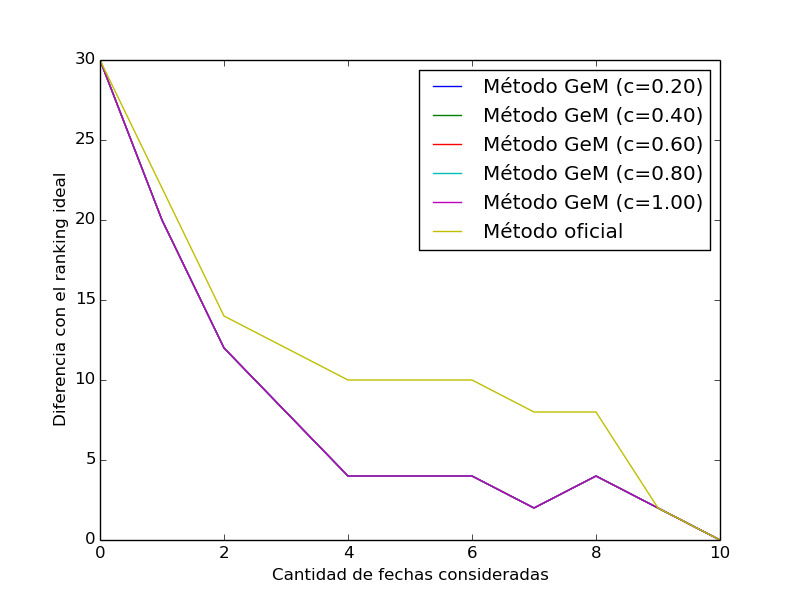
\includegraphics[width=.5\textwidth]{exp5_10_equipos.png}
    }
    \subfloat[][Torneo de 50 equipos]{
        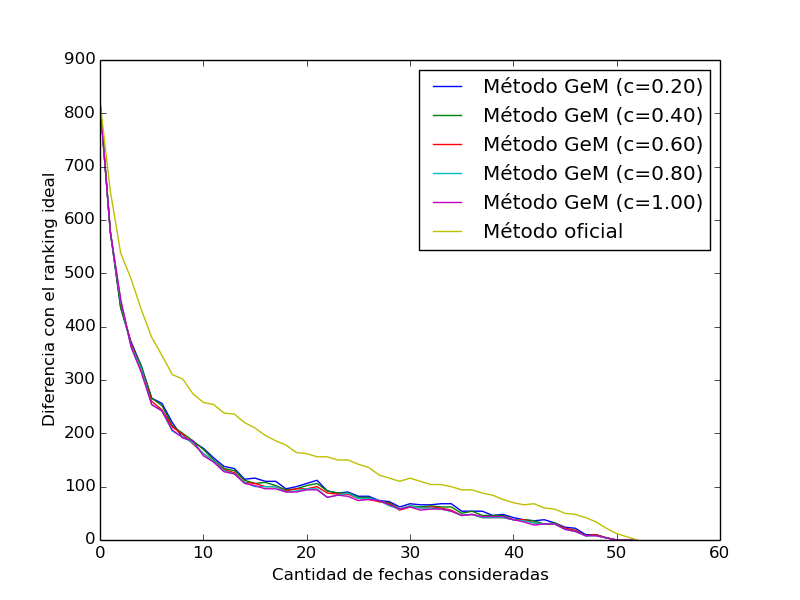
\includegraphics[width=.5\textwidth]{exp5_50_equipos.png}
        \label{subfig:exp5_50equipos}
    }
\end{figure}

\par La hip\'otesis fue confirmada. GeM converge al Orden Real para todos los
valores no nulos de $\alpha$ y no precisa todas las fechas para hacerlo, como se
puede observar en la figura \ref{fig:exp5_1}. Sin embargo, necesita una cantidad
significativa: para todos los valores no nulos de $\alpha$ fueron necesarias 10
de 11 fechas para el caso de 10 equipos y 50 de 53 fechas para el caso de 50
equipos.

\par El caso $\alpha=0$ no funciona porque la matriz termina descartando los
resultados de los equipos y usando simplemente la misma probabilidad para
cualquier equipo. En adelante dejaremos de lado este caso.

\par La variaci\'on $\alpha$ en el caso de 10 equipos no represent\'o
diferencias en el orden devuelto en cada fecha. es por eso que en la figura
\ref{subfig:exp5_10equipos} no se ven m\'as que dos curvas (una de las cuales
corresponde al siguiente experimento): estan todas superpuestas. En el caso de
50 equipos s\'i hubo leves diferencias en el orden devuelto en cada fecha.
Observamos que a mayor $\alpha$ el algoritmo en general converge ''mejor'' al
Orden Real (es decir, dada la misma cantidad de fechas, se acerca m\'as), aunque
siempre precisa 50 fechas para converger al orden real (figura
\ref{subfig:exp5_50equipos}). La diferencia de todos modos es peque\~na y probablemente se deba a que, en
nuestro modelo ideal, las victorias son totalmente transitivas: la probabilidad
de que $C$ le gane a $A$ dado que $A$ le gan\'o a $B$ y $B$ le ganó a $C$ es
siempre $0$.  Como valores peque\~nos de $\alpha$ tienden a agregar una
probabilidad de que $C$ efectivamente le gane a $A$, la convergencia mejora
levemente para valores altos de $\alpha$ (donde esa probabilidad artificial es
cada vez menor). Sin embargo, variando la semilla usada para ordenar los
enfrentamientos encontramos casos en donde un valor mayor de $\alpha$ empeoraba
la convergencia en alg\'un punto (ver figura \ref{subfig:exp5_c_malo}), por lo
que no podemos generalizar esta conclusi\'on.

\par As\'i pues, motivados por estos resultados, realizamos la siguiente
experimentaci\'on.

%---------------------------------------------------------------
\subsubsection*{PageRank vs Ranking FIFA en un caso de Orden Total Conocido}
\label{subsec:exp5_aux}
\begin{LaTeXdescription}
    \item[Objetivo] Comparar GeM contra el raking est\'andar del f\'utbol en un
        caso ideal.\\

    \item[Hip\'otesis] PageRank, utilizando el modelo GeM, converge m\'as
        r\'apido al ''Orden Real'', si lo hay, que el sistema oficial del
        f\'utbol asociado establecido por la FIFA\cite{fifa}.\\

    \item[Proposici\'on] Asumiendo que se confirm\'o la hip\'otesis del
        experimento anterior, nos interesa analizar si, asumiendo que existe un
        orden ideal/correcto, GeM se comporta peor, igual o mejor que la forma
        est\'andar de ordenar a los equipos (por puntos, 3/1/0 puntos para
        victoria/empate/derrota) donde ''comportarse'' mejor significa que con
        la misma información disponible (por ejemplo, la mitad de los partidos
        jugados) se acerca m\'as al orden ideal.\\

    \item[M\'etodo de Experimentaci\'on] Consideramos las mismas instancias de
        prueba que el experimento anterior. Comparamos la distancia entre GeM y
        el orden ideal contra la distancia entre el ordenamiento est\'andar y el
        orden ideal, usando la misma definici\'on de distancia de rankings que
        para el experimento anterior y el mismo criterio para ordenar equipos
        empatados en puntaje. De confirmarse nuestra hip\'otesis, deber\'iamos
        ver que GeM se acerca ''m\'as r\'apido'', es decir, con menos fechas, al
        orden ideal.\\

    \item[Resultados, an\'alisis y discusi\'on] 
\end{LaTeXdescription}

\begin{figure}[H]
    \caption{Casos Patol\'ogicos (10 equipos, $c = \alpha$)}
    \label{fig:exp5_2}
    \centering
    \subfloat[][Caso particular malo para $\alpha$ grande]{
        \label{subfig:exp5_c_malo}
        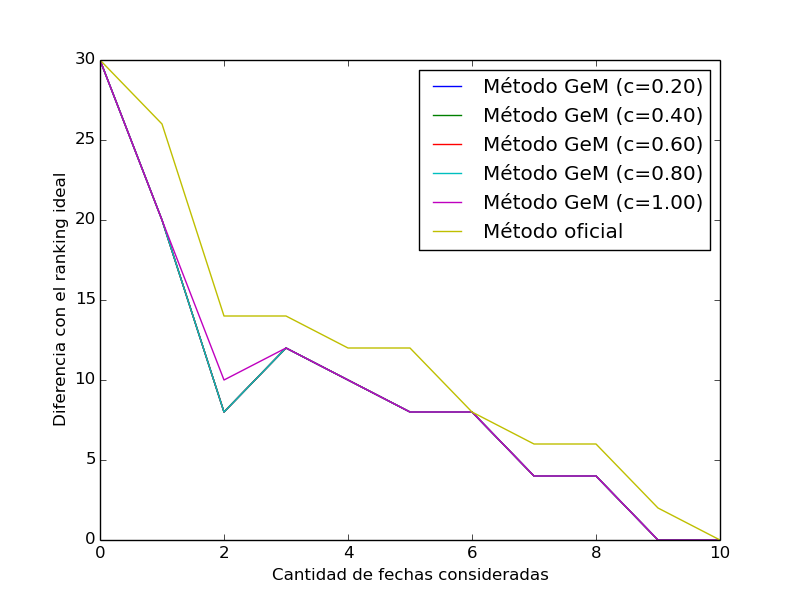
\includegraphics[width=.5\textwidth]{exp5_ejemplo_c_malo.png}
    }
    \subfloat[][Caso particular malo para GeM]{
        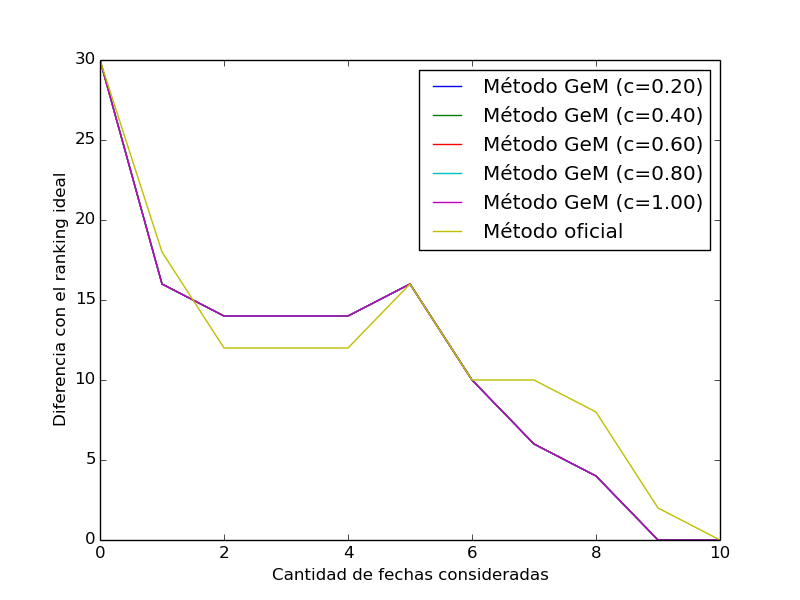
\includegraphics[width=.5\textwidth]{exp5_ejemplo_gem_malo.png}
        \label{subfig:exp5_gem_malo}
    }
\end{figure}

\par Comparamos GeM con el orden oficial, establecido por asignación de puntos
(3-1-0) y confirmamos tambi\'en nuestra hip\'otesis de que en el caso promedio,
GeM se comporta mejor que el orden oficial de asignaci\'on de puntajes,
acerc\'andose más al ideal para cualquier cantidad de fechas.

\par Sin embargo tambi\'en encontramos semillas para las cuales esto no era real
en alg\'un punto (ver figura \ref{subfig:exp5_gem_malo}) por lo que tampoco
podemos generalizar esta conclusi\'on.

\par Por \'ultimo, dado que los dos casos ''patol\'ogicos'' fueron encontrados
con la instancia de pocos equipos (10) y no logramos encontrar una semilla que
los genere en el caso de muchos (50), podr\'iamos argumentar que GeM se comporta
''mejor'' cuando la cantidad de equipos es grande. Queda fuera de los alcances
de este trabajo confirmar m\'as sistem\'aticamente esa hip\'otesis, pero es un
buen trabajo futuro.

%---------------------------------------------------------------
\medskip
\par En este experimento se trabaj\'o principalmente con instancias artificiales
''de juguete''. Las mismas lejos est\'an de representar la realidad, pero nos
sirvieron para poder asegurar que el modelo GeM ''descubrir\'ia'' el ranking
justo (o real, como dir\'ia Platon) si este existiese. A\'un as\'i, observamos
que para llegar a este ranking el modelo requerir\'a de mucha informaci\'on de
entrada, lo cual le quita quiz\'as utilidad como predictor de resultados de
torneos\footnote{Sin \'animo de menospreciar a GeM, si uno tiene los datos de 50
sobre 53 fechas, predecir con buena probabilidad de acierto el orden final no es
necesariamente una tarea extremadamente dif\'icil.}. Tambi\'en observamos que en
la progesi\'on fecha a fecha, el par\'ametro $\alpha$ pareciera tener de muy
poca a nula influencia sobre los rankings obtenidos.

\par Por \'ultimo, al comparar la ''velocidad de aproximaci\'on al ranking ideal'' con el sistema de puntaje real, pudimos ver que si
bien considerabamos no tan bueno a GeM para aproximarse con poca informaci\'on
al resultado final, se comporta mejor que el ranking oficial (para
los casos ideales que fueron considerados), con lo cual este modelo quiz\'as
podr\'ia ser un primer paso hacia un predictor de resultados de torneos de
f\'utbol profesional\footnote{Y la dominaci\'on mundial.}.


\newpage
\subsubsection{GeM vs Ranking Oficial}
\label{subsec:exp6}
\begin{LaTeXdescription}
    \item[Objetivo] Comparar GeM con los rankings estándar en el mundo real.\\

    \item[Proposici\'on] En la vida real la emoción subyacente de los deportes
        radica, en parte, en la posibilidad de que cualquiera le gane a
        cualquiera. ¿Para qué practicar u observar/seguir un deporte si este no
        es el caso?  Un ranking trata de dar un orden que determine que
        participante es mejor que otro entre los que forman parte de una
        competición. Pero la confección de este ranking puede tener que variar
        de acuerdo a la forma de la competición: no en todos los eventos todos
        los equipos juegan contra todos, no siempre todos juegan la misma
        cantidad de partidos ni la misma cantidad de veces entre sí. Así pues,
        dar un ranking se vuelve más complicado. Nuestra idea es tomar casos del
        mundo real y observar los resultados de GeM y ver cómo se comporta
        respecto de estas asimetrías inherentes al tipo de competición; mientras
        que lo comparamos contra el ranking oficial utilizado en cada caso.\\

    \item[M\'etodo de Experimentaci\'on] Evaluaremos 3 instancias de
        deportes/ligas:

        \begin{enumerate}
            \item El campeonato de Primera División del fútbol argentino 2015,
                tomando hasta la fecha 23.

            \item La Copa Mundial de la FIFA de 2014, realizada en Brasil.

            \item La Copa Mundial de la FIFA de 1954, realizada en Suiza.
        \end{enumerate}
        \medskip

        \par Tomamos el campeonato argentino como un ejemplo del formato de
        liga, y las Copas Mundiales de Fútbol como un ejemplo del caso en que no
        juegan todos contra todos ni todos juegan la misma cantidad de veces.
        Tomamos el caso de 2014 como representante del formato ''actual'' de 32
        equipos con una única fase de grupos y una fase eliminatoria. Y tomamos
        el caso de 1954 por presentar una situación interesante de analizar: en
        la fase de grupos Hungría le ganó 8 a 3 al que luego saldría campeón,
        Alemania Federal.

        \par Para los casos de los Mundiales, tomamos como ''oficial'' el
        ranking final publicado por la FIFA. Para el caso del campeonato de
        primera división, la ordenación estándar por puntaje 3-1-0.

        \par En los tres casos ejecutamos el algoritmo GeM variando los valores
        de $\alpha$ y comparamos contra el ranking oficial de la instancia. En
        los tres casos decidimos ignorar los empates. Para las definiciones por
        tanda de penales, tomamos como resultado del partido el resultado final
        de los mismos.\\

    \item[Resultados, an\'alisis y discusi\'on]
\end{LaTeXdescription}

%%*************************************************************************
\begin{enumerate}[parsep=1ex]
    \item Lo primero que notamos es que para valores grandes de $\alpha$ la
        diferencia con el ranking oficial aumenta, alcanzando un mínimo en
        $\alpha=0.1$. Consideramos que esto tiene que ver por darle demasiada
        importancia a la ''transitividad de victorias'' cuando el fútbol en
        general no funciona de esa manera. Por ejemplo, para $\alpha=1$ los
        primeros cinco puestos son:

        \begin{figure}[H]
            \centering
            \subfloat[][Primeros Puestos\label{subfig:exp6_arg}]{
                \footnotesize
                \setlength{\tabcolsep}{3pt}
                \begin{tabular}[b]{|l|r||l|r|}
                    \hline
                    \multicolumn{2}{|c||}{GeM}&\multicolumn{2}{c|}{Oficial: 3-1-0}\\
                    \hline
                    Equipo & Puntaje & Equipo & Puntaje\\
                    \hline\hline
                    Boca Juniors &0.0934262& San Lorenzo &50 \\
                    River Plate &0.0828491& Boca Juniors &49 \\
                    San Martín (SJ) &0.0674819& Racing Club &46 \\
                    Aldosivi &0.0648027& Rosario Central &45 \\
                    San Lorenzo &0.0596129& River Plate &44 \\
                    \hline
                \end{tabular}
            }\hspace{10pt}
            \subfloat[][Diferencia en funci\'on de $\alpha$\label{subfig:exp6_arg_diff}]{
                \raisebox{-0.2\height}{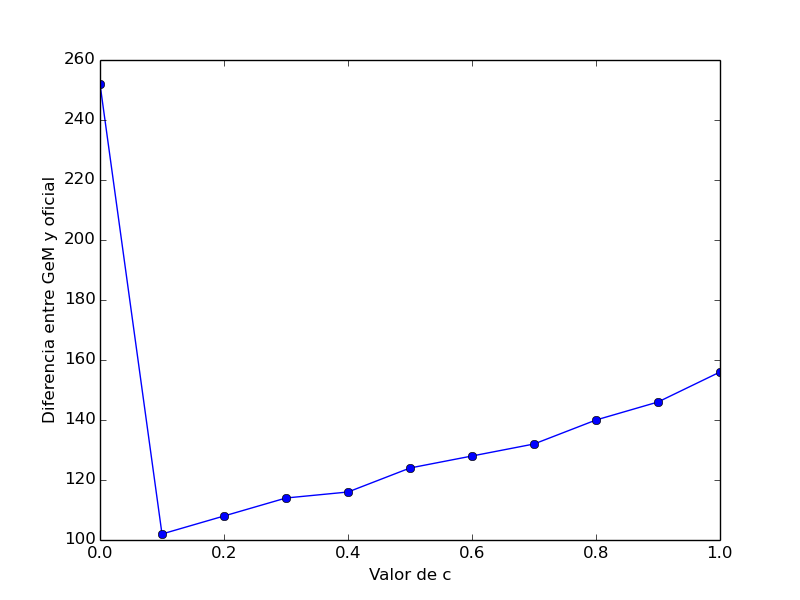
\includegraphics[width=.5\textwidth]{exp6_arg.png}}
            }
            \caption{GeM vs Primera Divisi\'on F\'utbol Argentino para $\alpha=1$}
            \label{fig:exp6_arg_1}
        \end{figure}

        \par La posición de San Martín de San Juan (13º según el puntaje
        oficial) en el ranking GeM se debe, en parte, a que le ganó a San
        Lorenzo en la fecha 3, mientras que Aldosivi (24º según el puntaje
        oficial) logró lo mismo en la fecha 10 y le gano a San Martín de San
        Juan en la fecha 22. Removiendo esos partidos sus posiciones en GeM
        bajan significativamente.

        \par De todos modos podemos observar que, para el valor de $\alpha=0.1$,
        el ranking devuelto por GeM se parece un poco más al oficial, d\'andonos
        los 6 primeros puestos que se pueden observar en el cuadro
        \ref{subfig:exp6_arg_prim}.

        \begin{figure}[H]
            \centering
            \subfloat[][Primeros Puestos\label{subfig:exp6_arg_prim}]{
                \footnotesize
                \setlength{\tabcolsep}{3pt}
                \begin{tabular}{|l|r||l|r|}
                    \hline
                    \multicolumn{2}{|c||}{GeM}&\multicolumn{2}{c|}{Oficial: 3-1-0}\\
                    \hline
                    Equipo & Puntaje & Equipo & Puntaje\\
                    \hline\hline
                    River Plate &0.0383429& San Lorenzo &50 \\
                    Boca Juniors& 0.038337& Boca Juniors &49 \\
                    San Lorenzo &0.0372973& Racing Club &46 \\
                    Racing Club &0.0363868& Rosario Central &45 \\
                    San Martín (SJ) &0.0352285& River Plate &44 \\
                    Rosario Central &0.0347587& Independiente &38\\
                    \hline
                \end{tabular}
            }\hspace{2pt}
            \subfloat[][\'Ultimos Puestos\label{subfig:exp6_arg_ult}]{
                \footnotesize
                \setlength{\tabcolsep}{3pt}
                \begin{tabular}{|l|r||l|r|}
                    \hline
                    \multicolumn{2}{|c||}{GeM}&\multicolumn{2}{c|}{Oficial: 3-1-0}\\
                    \hline
                    Equipo & Puntaje & Equipo & Puntaje\\
                    \hline\hline
                    Olimpo &0.0316438&Godoy Cruz &22\\
                    Huracán &0.0315532&Huracán &21\\
                    Godoy Cruz &0.0315278&Atlético de Rafaela &20\\
                    Atlético de Rafaela &0.0309498&Arsenal &17\\
                    Colón &0.0308694&Nueva Chicago &14\\
                    Nueva Chicago &0.0307189&Crucero del Norte &14\\
                    \hline
                \end{tabular}
            }
            \caption{GeM vs Primera Divisi\'on F\'utbol Argentino para $\alpha=0.1$}
            \label{fig:exp6_arg_2}
        \end{figure}
        \medskip

        \par De estos 6 primeros puestos de GeM, 5 efectivamente corresponden a
        esos primeros 6 lugares según el oficial (el que falta es Independiente,
        que GeM ubica 15º) y uno de ellos está en la misma posición en ambos
        rankings.

        \par Otra coincidencia notable son los últimos puestos, los cuales se
        pueden observar en el cuadro \ref{subfig:exp6_arg_ult}. Esta tabla tiene
        3 coincidencias débiles (mismos equipos en distinta posición) y una
        coincidencia exacta.\\

%%*************************************************************************
    \item En este caso, la diferencia para valores no nulos de $\alpha$ 
        es escasa, y la diferencia con el oficial en general es mucho mejor que
        para el caso del campeonato argentino. Consideramos esto relacionado al
        hecho de que hay pocos partidos en total, y a que la organización del
        torneo también se basa fuertemente en la transitividad de victorias (al
        menos en la fase final): en un Mundial, si A le ganó a B y B a C, se asume que A es
        mejor que C.

        \par Para todos los valores no nulos de $\alpha$ GeM ubicó
        correctamente como ganador a Alemania. Para $\alpha=0.1$ considero que
        el subcampeón fue Países Bajos, lo cual sorprende dado que Argentina le
        ganó ''4 a 2'' (el resultado de los penales). Evidentemente un valor tan
        bajo de $\alpha$ le da baja importancia a esto y pondera más las
        diferencias de goles de Países Bajos contra sus rivales (4 vs España, 2
        vs Chile), mucho mejores que las de Argentina (que ganó todos sus
        otros partidos por un gol de diferencia). Para todos los demás valores de
        $\alpha$, GeM identificó correctamente a Argentina como subcampeón.

        \par Las menores diferencias generales se obtuvieron para $\alpha=0.2$,
        $\alpha=0.3$ y $\alpha=0.4$ ''empatadas'' en una distancia de 50 con el
        ranking oficial de la FIFA. En estos casos sorprende la precisión de los
        resultados. Por ejemplo, observemos los primeros 8 lugares en la
        siguiente tabla, que coinciden exactamente con el ranking provisto por
        la FIFA:

        \begin{figure}[H]
            \centering
            \subfloat[][Primeros puestos $\alpha=0.4$]{
                \footnotesize
                \setlength{\tabcolsep}{3pt}
                \begin{tabular}[b]{|l|r|}
                    \hline
                    Equipo & Puntaje\\
                    \hline\hline
                    Alemania &0.0986858\\
                    Argentina &0.0764719\\
                    Países Bajos &0.0650904\\
                    Brasil &0.0480157\\
                    Colombia& 0.0419815\\
                    Bélgica &0.0405001\\
                    Francia &0.0396461\\
                    Costa Rica &0.0344357\\
                    \hline
                \end{tabular}
            }\hspace{10pt}
            \subfloat[][Diferencia en Funci\'on de $\alpha$]{
                \raisebox{-.13\height}{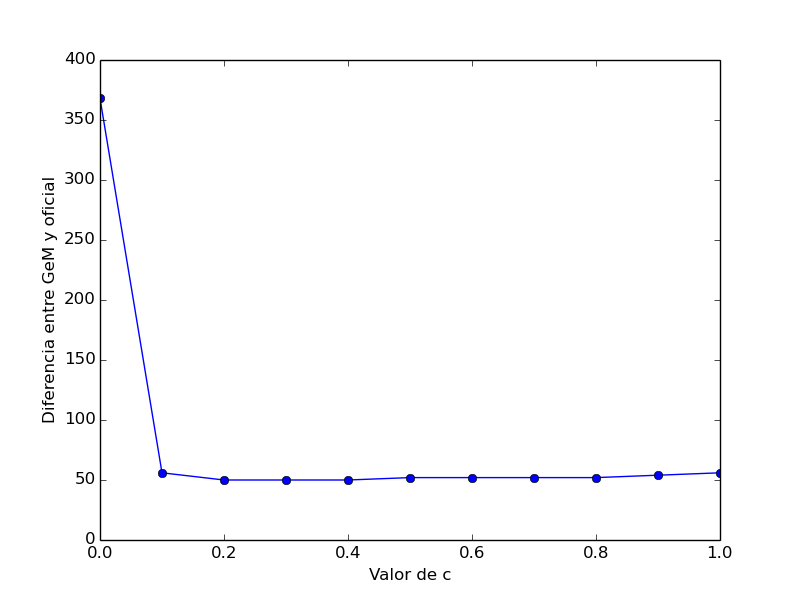
\includegraphics[width=0.5\textwidth]{exp6_2014.png}}
            }
            \caption{GeM vs Copa del Mundo 2014}
        \end{figure}

        Al consultarle su opinión al respecto de si fue o
        no penal, GeM guardó un respetuoso silencio.

%%*************************************************************************
    \item Nuevamente observamos una buena aproximación entre GeM y el ranking
        oficial. Quizás los más sorprendente es que para todos los valores no
        nulos de $\alpha$, GeM supo clasificar a Alemania Federal como el
        ganador del torneo a pesar de haber perdido por una diferencia de 5
        goles en la fase de grupos con el subcampeón Hungría. La explicación que
        le encontramos a esto se basa en que la final se disputó precisamente
        entre esos dos equipos, y Alemania Federal se consagró ganador por 3 a
        2. Esto produce que el grafo de conectividad tenga un ciclo entre esas
        dos selecciones, lo cual hace que parte del "puntaje" de Hungría vuelva
        a Alemania Federal. Todo eso sumado a la excelente campaña de este
        último en el campeonato (4 a 1 vs Turquía, 7 a 2 nuevamente vs Turquía,
        2 a 0 vs Yugoslavia y 6 a 1 vs Austria, que venía de ganar varios
        partidos también por gran diferencia) lo posiciona efectivamente como
        ganador según GeM.

        \par También para todos los valores de $\alpha$ GeM acierta en ubicar a
        Hungría como subcampeón.

        \par La menor diferencia con el ranking oficial se obtiene con
        $\alpha=0.8$ y $\alpha=0.9$. Es preciso notar que no pudimos evaluar el
        caso $\alpha=1$ por no converger para esta instancia, a diferencia de
        las dos competiciones anteriores\footnote{Sabemos por la secci\'on
        \ref{sec:introduccion} que la convergencia está asegurada solo para $0\leq\alpha <1$, pero de todos modos venimos
        ``ensayando'' con $\alpha=1$ sabiendo que dicho valor no tiene por qué hacer
        converger al m\'etodo de la potencia para nuestro $M$}.

        \par En estos dos casos, GeM acertó en los 5 primeros puestos de la
        competición, siendo estos:

        \begin{figure}[H]
            \centering
            \subfloat[][Primeros Puestos $\alpha=0.4$]{
                \footnotesize
                \setlength{\tabcolsep}{3pt}
                \begin{tabular}{|l|r|}
                    \hline
                    Equipo & Puntaje\\
                    \hline\hline
                    Alemania Federal &0.421402\\
                    Hungría &0.409884\\
                    Austria &0.0299615\\
                    Uruguay &0.0252637\\
                    Suiza &0.0169375\\
                    \hline
                \end{tabular}
            }\hspace{10pt}
            \subfloat[][Diferencia en Funci\'on de $\alpha$]{
                \raisebox{-.5\height}{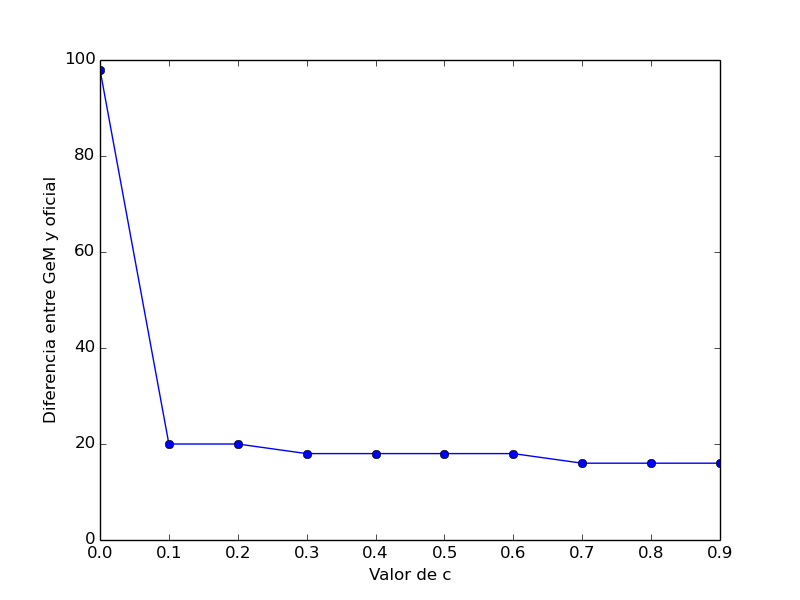
\includegraphics[width=0.5\textwidth]{exp6_1954.png}}
            }
            \caption{GeM vs Copa del Mundo 1954}
        \end{figure}
\end{enumerate}
\medskip

%%*************************************************************************
\par Lo m\'as jugoso de toda esta experimentaci\'on radica en que comparamos el
modelo GeM de rankings contra todos rankings oficiales que est\'an vigentes. El
primer resultado interesante es observar que GeM est\'a mucho m\'as cerca para
del ranking utilizado en las copas del mundo que del torneo actual del f\'utbol
argentino, y esto se ve para cualquier $\alpha\neq 0$ (el caso con $\alpha = 0$,
como ya se comentado en experimentos previos, concibe un modelo donde todos los
equipos le pueden ganar a todos con la misma probabilidad, sin importar los
resultados previos, haciendo a este par\'ametro poco interesante para analizar
por su obvia ignorancia de la realidad\footnote{¿O acaso las chances de que
Racing le gane a Crucero del Norte son las mismas de que pierda?}). A\'un as\'i,
a pesar de esta distancia, vemos que en el caso del torneo de f\'utbol
argentino, su ranking en los extremos de la ''tabla'' (particularmente en el
extremo inferior) suele ubicar a los mismos equipos que el ranking oficial. Esto
nos indica que a pesar de tener rankings muy distintos, en t\'erminos generales
ambos rankings diferencian de forma similar a los equipos ''buenos'' y
''malos''.

\par Concluyendo, vemos que GeM puede o no parecerse a otros rankings oficiales,
pero la determinaci\'on de si es mejor o peor depender\'a de qué opinen quienes
lo utilicen. Lo que si podemos afirmar es que GeM tiende a aproximarse m\'as
a los rankings oficiales (al menos los vistos) en los extremos del mismo. Es
decir, a pesar de estar a una distancia no despreciable del ranking oficial, los
equipos se\~nalados como los m\'as fuertes o mejores por ambos rankings (o los
peores) tienen varias coincidencias. Decimos entonces que, desde el punto de
vista de clasificar a un equipo como ''de los buenos'' o ''de los malos'' de la
competencia, cualquiera de los rankings dar\'ia resultados similares, pero estos
se diferencian al entrar en el detalle de qué equipo es mejor que otro.


\newpage
\subsubsection{Estabilidad de GeM}
\label{subsec:exp7}
\begin{LaTeXdescription}
    \item[Objetivo] Observar el ranking de PageRank/GeM puede sufrir variaciones
        importantes de una fecha a la otra, al recibir un set nuevo de
        informaci\'on.\\

    \item[Hip\'otesis] GeM es m\'as inestable que la puntuaci\'on oficial del
        f\'utbol.\\

    \item[Proposici\'on] Nos interesa considerar casos extremos para evaluar la
        estabilidad del ranking que devuelve GeM. El sistema de puntaje actual
        del f\'utbol tiene la caracter\'istica de ser bastante ''estable'': en
        una \'unica fecha un equipo puede ganar a lo sumo 3 puntos, lo cual
        (salvo en los comienzos de un torneo o casos de empate m\'ultiple
        dif\'iciles de encontrar en la realidad) no lo hace avanzar m\'as de 4 o
        5 posiciones.

        \par Nos interesa analizar si esta propiedad se conserva en GeM. Para
        eso, imaginemos un torneo de f\'utbol desbalanceado, es decir, un torneo
        en que al finalizar, el primer equipo tiene mucha diferencia con el
        \'ultimo\footnote{Consideramos esto desbalanceado. Si no es este el
        caso del lector, simplemente considerar una instancia que cumpla con esa
        condici\'on.}. Si en una \'ultima fecha ''inventada'', agregada
        artificialmente, el \'ultimo le ganase al primero, el m\'etodo de
        puntuaci\'on est\'andar dif\'icilmente altere demasiado el ranking.
        Queremos observar si esto ocurre con GeM.\\

    \item[M\'etodo de Experimentaci\'on] Tomamos el Campeonato de Primera B
        Nacional 2013/14, en el cual Banfield (1º) termin\'o con 78 puntos
        mientras que Villa San Carlos (22º y \'ultimo) termin\'o con 24.
        Generamos una fecha artificial extra en la que Villa San Carlos le gana
        a Banfield. El ranking oficial no cambiar\'ia, dado que con 27
        puntos Villa San Carlos seguir\'ia \'ultimo. De confirmarse nuestra
        hip\'otesis, esperar\'iamos ver un cambio en la posición que GeM le
        asigna a Villa San Carlos. En este caso, variando la cantidad de goles,
        estudiamos cu\'anto se alterar\'ia el resultado si la victoria fuese
        m\'as abultada. El valor de $\alpha$ usado fue de 0.85.\\

    \item[Resultados, an\'alisis y discusi\'on]
\end{LaTeXdescription}

\par Se confirmó la hipótesis. Efectivamente GeM altera el ranking por una
simple victoria por 1 a 0, aunque Villa San Carlos sigue último. Esto se debe a
que el puntaje GeM de Banfield cae y el de VSC sube, alterando a los demás
equipos que ganaron o perdieron contra alguno de ellos.

\begin{figure}[H]
    \centering
    \subfloat[][Distancia GeM Adulterado vs Oficial/GeM\label{subfig:exp7_dist_ranks}]{
        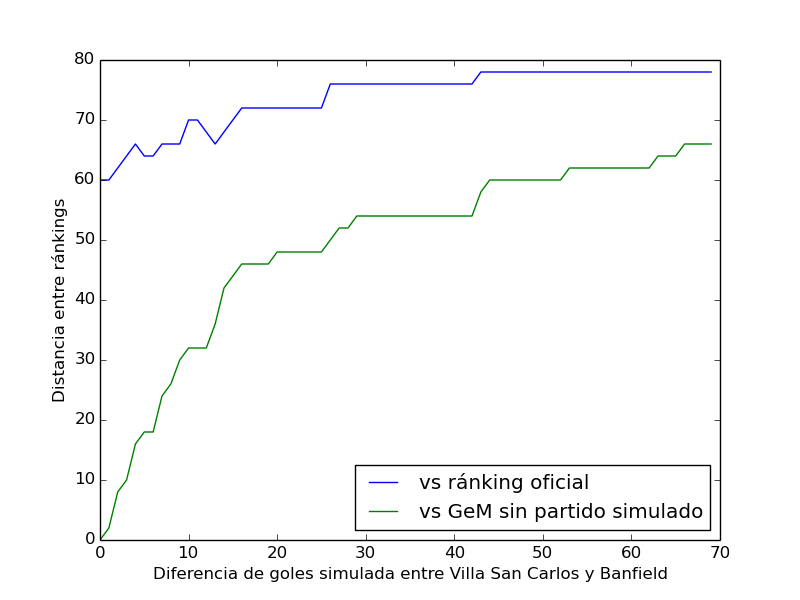
\includegraphics[width=.45\textwidth]{exp7_diferencia_ranks_funcion_goles.png}
    }\hspace{2pt}
    \subfloat[][Posición de Villa San Carlos en GeM Adulterado\label{subfig:exp7_pos_vsc}]{
        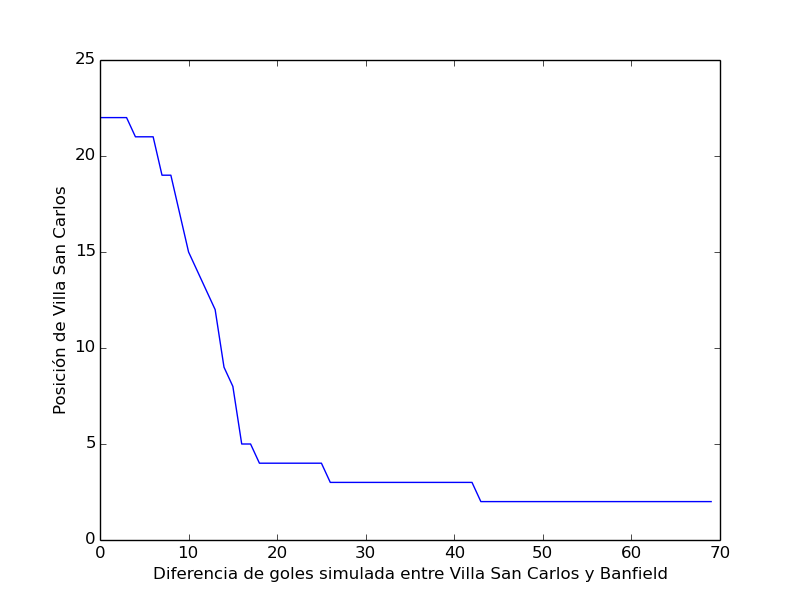
\includegraphics[width=.45\textwidth]{exp7_poscion_villa_san_carlos.png}
    }
    \caption{Consecuencias de introducir un partido artificial}
\end{figure}

\par Alcanza con una victoria de 4 a 0 para que Villa San Carlos deje el último
lugar. Y con una victoria de 43 a 0 pasa a estar en 2do lugar. Si esto parece
irreal, considerar el récord del fútbol profesional de goles en un mismo
partido: \emph{AS Adema 149 - 0 SO l'Emyrne}, el 31 de octubre de 2002 por la
\emph{THB Champions League de Madagascar}\footnote{En honor a la verdad, este
resultado fue alcanzado por goles en contra por protesta contra el arbitraje.
El resultado ``honesto'' más abultado fue \emph{Arbroath FC 36 - 0 Bon Accord
FC}, el 12 de septiembre de 1885 por la Copa Escocesa 1885-86 y, más
recientemente, el conocido \emph{Australia 31 - 0 Samoa Americana}, el 11 de
abril de 2001, por la clasificación al Mundial de Fúbol Corea-Japón 2002}.

\par En la figura \ref{subfig:exp7_pos_vsc} se puede observar la posición de
Villa San Carlos en función de la cantidad de goles del partido artificial. En
la figura \ref{subfig:exp7_dist_ranks} se puede observar la diferencia entre
rankings producida por el partido simulado en función de la cantidad de goles
del partido. Se observa claramente la ``inestabilidad'' de la que hablábamos:
por los resultados de un simple partido GeM puede alterar el orden en un factor
grande. Consideramos que esta no es una propiedad deseable del sistema, al
menos no para el fútbol: hay muchos factores que influyen en un resultado,
independientemente de la calidad de los competidores (azar, arbitraje, clima,
estado del campo, etc.). Un equipo ``malo'' no debería dejar de serlo solo por
haber haber tenido suerte (o incluso por haber hecho un único buen partido)
contra un equipo ``bueno'', o porque su rival haya hecho un partido malo.

\par El próximo experimento apunta a dejar aún más en evidencia esta situación.


\newpage
\subsection{Caso Particular GeM}
\label{subsec:exp8}
\begin{LaTeXdescription}
    \item[Objetivo] Analizar cuan ``justo'' es GeM, para un caso particular en
        el cual no haya dudas sobre lo que es justo y lo que no\footnote{O que
        haya muy poca probabilidad de que haya dudas al respecto.}.\\

    \item[Proposici\'on] Nos interesa analizar cu\'an ''justo'' es GeM para
        cierta definici\'on de justicia. Consideremos el caso de un torneo en
        que el equipo A le gana a todos los equipos salvo a B, y B pierde todos
        los partidos salvo el que le gana a A. Bajo nuestra definición de
        ''justicia'' o ''equidad'', o un aspecto de ella, A deber\'ia estar
        seguro por encima de B y B no deber\'ia estar por encima de muchos
        equipos (ya que perdi\'o contra todos). Observamos que en el caso del
        f\'utbol y su ránking 3-1-0 (o el esquema antiguo, 2-1-0) efectivamente
        B estar\'ia en la \'ultima posici\'on y A estar\'ia en la primera
        (eventualmente compartiendo dichas posiciones con alg\'un otro equipo).
        Entendemos entonces que este caso particular el ranking 3-1-0 es
        ''justo'' en este aspecto. Pero intu\'imos que esto no ser\'a lo que
        ocurra con GeM, ya que en el grafo de la instancia, A tiene un \'unico
        eje saliente (hacia B) y 18 entrantes, con lo cual su arista deber\'ia
        hacer subir mucho a B en el ranking.\\

    \item[Hip\'otesis] PageRank/GeM no es ''justo'' en cuanto al aspecto
        mencionado.\\

    \item[M\'etodo de Experimentaci\'on] Generamos una instancia de 20 equipos
        todos contra todos, donde existen A y B como se describieron. Entre los
        dem\'as equipos hacemos que el ganador sea aleatorios (con semilla =
        5). Todos los partidos terminan 1 a 0. Ejecutamos GeM y observamos el
        ranking final para diferentes valores de $\alpha$ (el factor de
        navegaci\'on).

    \item[Resultados, an\'alisis y discusi\'on] Lo primero que observamos es que B no ascendió al primer lugar para ningún valor de $\alpha$, lo cual era esperable dados los resultados del experimento 7 pero no deja de darnos cierta ``tranquilidad''. Sin embargo, y como se puede ver en la figura \ref{fig:exp8_posB}, la posición del equipo B sí mejora significativamente ya para valores pequeños de $\alpha$: ya un valor de $\alpha = 0.1$ deja a B 6to en el ránking, y a partir de $\alpha = 0.4$ pasa a estar 2do. Consideramos entonces que se confirmó nuestra hipótesis en el sentido de que GeM no es ``justo'' en un caso del estilo. Como ya postulamos en el experimento 7, no parece ``justo'' que un equipo prácticamente invicto que tuvo un ``mal día'' le permita a otro equipo salir 2do en una competencia en la que perdió con cuanto rival se cruzó.
    
    Podemos concluir entonces que los valores más ``justos'' de $\alpha$ serían los más bajos, dado que le dan menos importancia a estas situaciones extrañas pero perfectamente posibles en cualquier deporte.
    
\end{LaTeXdescription}

\begin{wrapfigure}{l}{0.5\textwidth}
    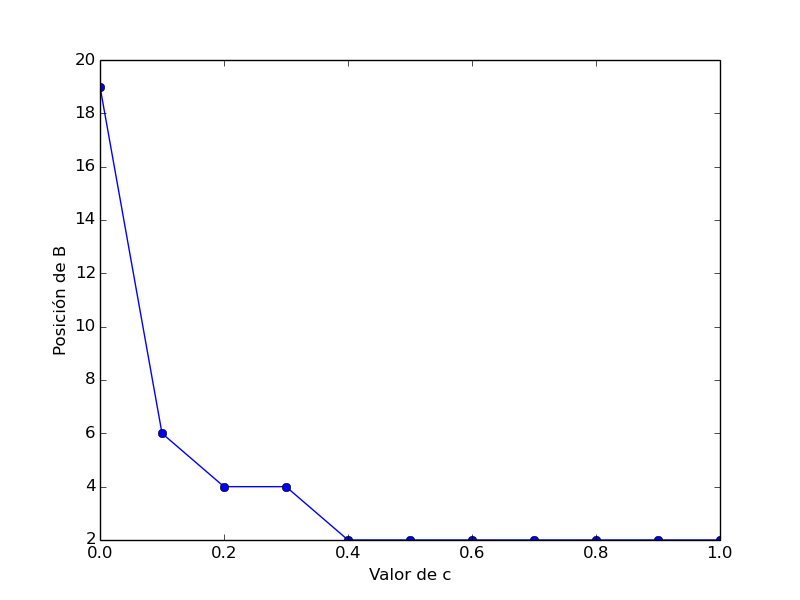
\includegraphics[width=0.5\textwidth]{exp8_posicion_B.png}
    \caption{Posici\'on del equipo B en el ranking en funci\'on del factor
        $\alpha$ ($c=\alpha$)}
    \label{fig:exp8_posB}
\end{wrapfigure}
\noindent

%---------------------------------------------------------------

\newpage
\subsection*{Experimentos a Futuro}
\par Como experimentos futuros relacionados con estos temas, que por cuestiones
de tiempo y alcance de este trabajo no fueron realizados, quedaría evaluar la
\emph{sensibilidad} de PageRank y su convergencia al orden m\'as que al
(auto)vector de distribuci\'on estacionario.

\par En primer caso, la sensibilidad para PageRank, trata de exponer si cambios
peque\~nos en un grafo dado (algunos ejes menos, algunos ejes m\'as) modifican
radicalmente el orden obtenido. Y tambi\'en experimentar sobre como $\alpha$
afecta a esta sensibilidad.

\par En cuanto al caso de la convergencia al \'orden m\'as que al vector
resultante, lo que queremos explicar es que en realidad lo que se busca obtener
con PageRank es un ranking, m\'as all\'a de los puntajes de cada p\'agina web.
Quizás se podr\'ia observar si para toda instancia y $\alpha$ fijo, se puede
estimar estadist\'icamente que luego de $k$ iteraciones (que esperamos que sea
un n\'umero, o incluso una funci\'on que tome ciertos parametros y devuelva un
n\'umero, mucho menor que la cantidad de interaciones necesarias por el
m\'etodo para converger) ya se lleg\'o al mismo orden al que se llegar\'a al
converger (aunque con distintos puntajes). Si esto se pudiera realizar,
podr\'iamos tener una primera heur\'istica para mejorar el tiempo de
convergencia, aunque claramente estar\'iamos trabajando ya con orden \'aun m\'as
aproximado que el que devuelve el m\'etodo de la potencia implementado sobre
aritm\'etica finita.
